\renewcommand{\lastmod}{September 18, 2023}
\renewcommand{\chapterauthors}{Markus Lippitz}

\chapter{Fourier Optics}

\section{Overview}
Fourier transformation simplifies the description of light, especially when it passes through obstacles, as in diffraction. The action of a lens also involves a Fourier transform. This is the field of \emph{Fourier optics}. I will follow chapter 4 of \cite{SalehTeich1991} here. Another good source is \cite{Goodman2005}. Note that books (as Saleh \& Teich) from the engineering  side of optics use $j = - i = - \sqrt{-1}$ instead of $i$. Sometimes this $j$ is even written as $i$, so engineering is the complex conjugate of physics.


We will briefly lay the foundations of Fourier optics and then discuss diffraction and optical Fourier transform through a lens. For our purposes it is sufficient to consider scalar waves, i.e. we ignore the vectorial nature of the electric (or magnetic) field of light and use only a complex scalar value at each point in space to describe light.

\section{Spatial frequencies}

Let us start with a plane wave
\begin{equation}
    U(\br) = A e^{i \bk \cdot \br} \quad \text{with} \quad k = | \bk | = \frac{2\pi}{\lambda} \quad .
\end{equation}
We assume that all three components of $\bk$ are real (\emph{far-field optics} in contrast to \emph{near-field optics}), but the amplitude $A$ might be complex.
The wave vector $\bk$ makes the angles $\Theta_{x,y}$ with the $x$--$z$ and the $y$--$z$ plane, respectively, with
\begin{equation}
    \sin \Theta_x = \frac{k_x}{k} \quad .
\end{equation}
In the $z=0$ plane, the field is
\begin{equation}
  U(x,y,0) = f(x,y) = A \, e^{2 \pi \, i (\nu_x x + \nu_y y) }
\end{equation}
with the \emph{spatial frequencies} $\nu_x$ and $\nu_y$ 
\begin{equation}
  \nu_{x,y} = \frac{k_{x,y}}{2 \pi} = \frac{1}{\Lambda_{x,y}}
\end{equation}
and the period of the field $\Lambda_{x,y}$ in the $x$ and $y$ direction. And of course all this is related, i.e.,
\begin{equation}
    \sin \Theta_x = \frac{k_x}{k} = \lambda \nu_x = \frac{\lambda}{\Lambda_x}
\end{equation}
and similar for the $y$ direction. The assumption of all-real $\bk$ components makes sure that for all combinations of $k_x$,$k_y$, $k_z$ an angle $\Theta$ can be found, i.e., the right side of the equation is real and below one in absolute value. 

We will almost always make the \emph{paraxial approximation} assuming that the wave vector is roughly parallel to the $z$-direction, the angles $\Theta_{x,y}$ are thus small, and $k_{x,y} \ll k$. Then we can omit the sine in the last equation and get 
\begin{equation}
     \Theta_x \approx \frac{k_x}{k} = \lambda \nu_x = \frac{\lambda}{\Lambda_x} \quad .
\end{equation}

What happened here? The combination of all-real $\bk$ components, i.e., optical far-field, and fixed wavelength $\lambda$ removes one degree of freedom in the three components of the wave vector. As long as we know the wavelength and we know that the plane wave is nicely propagating, only two  real values are enough to fully describe it. These two values could be the angles $\Theta_{x,y}$, or the spatial frequencies $\nu_{x,y}$ or the $\Lambda_{x,y}$.


\section{Transmittance function}

A plane wave of amplitude one is traveling in $+z$ direction. At $z=0$ it is transmitted through a thin optical element with the complex  transmittance function $f(x,y)$ with
\begin{equation}
    f(x,y) =  e^{2 \pi \, i (\nu_x x + \nu_y y) } \quad .
\end{equation}
Directly after this plate, the optical field is $U(x,y,0) = f(x,y)$, i.e., the field is modulated by the transmittance function. We know from above that such a field is traveling in the direction given by the $\Theta_{x,y}$ or equally by the spatial frequencies $\nu_{x,y}$. The field is thus diffracted in this direction.\sidenote{This is not an optical grating yet, as this would change the amplitudes only, i.e., have a real-valued tranmittance function.}

In general, if the transmittance function $f$ would have an arbitrary shape, it could be decomposed into a sum of harmonic functions. Each harmonic component would diffract a part of the plane wave into its direction. So when we express $f$ by its Fourier transform $F$
\begin{equation}
    f(x,y) = \mathcal{FT} \left\{ F(\nu_x, \nu_y) \right\}
     = \iint F(\nu_x, \nu_y)  \, e^{2 \pi \, i (\nu_x x + \nu_y y) } \, d\nu_x  d\nu_y
\end{equation}
then we get
\begin{equation}
    U(x,y,0) 
     = \iint F(\nu_x, \nu_y)  \, e^{2 \pi \, i (\nu_x x + \nu_y y) } \, d\nu_x  d\nu_y \quad .
\end{equation}
This becomes useful when calculating the field \emph{at any point in space}, i.e., by including the $z$ coordinate:
\begin{equation}
    U(x,y,z) 
     = \iint F(\nu_x, \nu_y)  \, e^{2 \pi \, i (\nu_x x + \nu_y y) } \,e^{i k_z z} \, d\nu_x  d\nu_y \quad ,
     \label{eq:2_Uxyz}
\end{equation}
where $k_z$ now depends on the integrating variables
\begin{equation}
    k_z = \sqrt{k^2 - k_x^2 - k_y^2} = 2 \pi \left( \frac{1}{\lambda^2} - \nu_x^2 - \nu_y^2 \right) \quad .
    \label{eq:2_Uxyz_kz}
\end{equation}
Again the requirement of propagating waves entails $\nu_x^2 + \nu_y^2 <  1/\lambda^2$, so not all Fourier components of $F$ play a role.


\section{Transfer function and impulse response}

Let us first introduce the concepts with electric  circuits such as an RC-filter. One can define a transfer function $H(\omega)$ that relates the frequency spectrum $F(\omega)$ at the input (of the filter) with that at the output 
\begin{equation}
    G(\omega) = F(\omega) \cdot H(\omega) \quad .
\end{equation}
In time domain, the impulse response $h(t)$ is another description. The signal $f(t)$ at the input results in an output $g(t)$
\begin{equation}
    g(t) = \int h(\tau) f(t - \tau) d\tau \quad ,
\end{equation}
where causality requires that $h(t)$ is zero for $t <0$. The interesting point is that not only the signals $f$ and $g$ are connected to their Fourier transforms $F$ and $G$, but also the transfer function $H$ is the Fourier transform of the impulse response $h$. A Fourier transform converts a product into a convolution, and vice versa.


\section{Transfer function of free space}

We now apply this scheme to spatial frequencies describing a superposition of plane waves. Letting the wave propagate by a distance $d$ from a source plane $f(x,y) = U(x,y,0)$ to a target plane $g(x,y) = U(x,y,d)$, how do the spatial amplitudes $F$ and $G$ relate? Looking at eq.  \ref{eq:2_Uxyz}, we see that it is just the last exponential function  that depends on $z$, but we need to take eq.  \ref{eq:2_Uxyz_kz} into account. Together we find
\begin{equation}
    H(\nu_x, \nu_y) = \exp \left(  
  2 \pi \, i  \, d \, \sqrt{ \frac{1}{\lambda^2} - \nu_x^2 - \nu_y^2 }
    \right) \quad .
\end{equation}
For spatial frequencies $\nu_x^2 + \nu_y^2 <  1/\lambda^2$, i.e., within a circle of radius $1/\lambda$, the magnitude does not change ($|H| = 1$), only the phase changes. Outside this circle, the magnitude drops exponentially width $d$, as the square-root becomes imaginary. These waves are called \emph{evanescent waves}, as they do not propagate and only exist in the near-field.

High spatial frequencies $\nu$ near $1/\lambda$ are far away from the paraxial approximation. In most cases it is sufficient to restrict ourself to low spatial frequencies $ \ll 1/\lambda$. In this case, we can use the \emph{Fresnel approximation} of the transfer function
\begin{equation}
    H(\nu_x, \nu_y)_\text{Fresnel} = H_0 \exp \left(  
   - 2 \pi \, i  \, d \, (
 \nu_x^2 + \nu_y^2 )
    \right) \quad \text{with} \quad H_0 = e^{i k d} \quad .
\end{equation}
The term $H_0$ factors out the trivial phase evolution due to propagation along the optical axis.

When we know the spatial frequency amplitudes $F$ at $z=0$, then we obtain $G$ at $z=d$ by
\begin{equation}
    G(\nu_x, \nu_y) =  F(\nu_x, \nu_y) \cdot  H(\nu_x, \nu_y) \quad .
\end{equation}
We can Fourier transform the equation to obtain 
\begin{equation}
    g(x,y) = f(x,y) \otimes h(x,y) \label{eq:2_gfh_conv}
\end{equation}
where $\otimes$ signals a convolution. The impulse response of free space is in the Fresnel approximation
\begin{equation}
    h(x,y)_\text{Fresnel} \approx h_0 \, \exp \left(i k \frac{x^2 + y^2 }{2d} \right) \quad \text{with} \quad
    h_0 = -\frac{i}{\lambda d} \,  e^{i k d } \quad .
\end{equation}
Eq. \ref{eq:2_gfh_conv} means that we get from one plane to the other by convolving each source point with a wave of shape $h$. This is equivalent to the Huygens principle, where each point should be a source of a spherical wave. When we take the paraxial approximation of a spherical wave we obtain $ h(x,y)_\text{Fresnel}$.


\section{Optical Fourier transform by propagation}

Up to now we used the Fourier transform to simplify description of optical fields. In this section, we will show that the propagation of an optical field by a long enough distance allows to optically 'compute' the Fourier transform. We will find that the field in the target plane $g(x,y)$ is proportional to the Fourier transform $F$ of the field in the source plane.

\begin{marginfigure}
    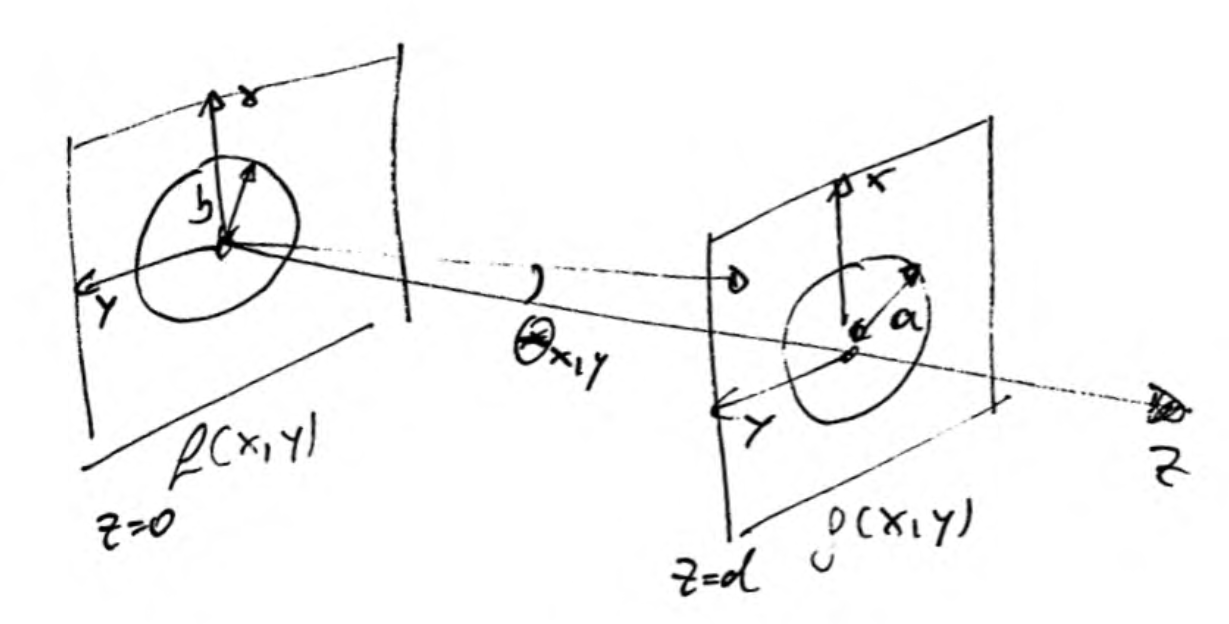
\includegraphics[width=\textwidth]{\currfiledir sketches/fraunhofer.png}
    \caption{Fraunhofer condition}
\end{marginfigure}

The Fourier components $F$ of the field $f$ in the source plane determine the direction of travel of the plane waves, as we have seen above. The problem is that a plane wave is everywhere in space. We need thus to find a condition for 'far enough' so that the individual pieces of the plane wave have separated enough. We do not only employ the paraxial approximation, i.e., that the wave vectors are not too inclined on the optical axis. The key point is that we also require the size of the source plane to be limited. This leads to the two conditions of the Fraunhofer approximation
\begin{equation}
    N_F =  \frac{a^2}{\lambda d} \ll 1 \quad \text{and} \quad
    N_{F}' =  \frac{b^2}{\lambda d} \ll 1 
\end{equation}
where the two $N_F$ are the Fresnel numbers, and $a$,$b$ are the radius of the relevant and allowed regions in the target and source planes, respectively. $d$ is again the distance between the  planes. The Fraunhofer approximation is a more severe restriction than the Fresnel approximation.

We start by writing down the convolution integral of eq. \ref{eq:2_gfh_conv} in the Fresnel approximation
\begin{align}
    g(x,y) = & f(x,y) \otimes h(x,y)_\text{Fresnel} \\
 = & h_0 \iint f(x', y') \,  \exp \left(i k \frac{(x-x')^2 + (y-y')^2 }{2d} \right)  \, dx' dy' \quad .
\end{align}
The term $(x-x')^2$ in the exponent of the exponential function is multiplied out into three terms. 
We keep the mixed terms. Both squared terms can be neglected due to the Fraunhofer approximation. For example  we get 
\begin{equation}
    \exp \left(i \pi  \frac{x'^2 + y'^2 }{ \lambda d} \right) \approx 1
\end{equation}
as  $N_{F}' \ll 1$. The terms without prime vanish due to $N_{F} \ll 1$. So we have
\begin{equation}
    g(x,y)  \approx h_0   
     \iint f(x', y') \,  \exp \left(-i 2 \pi \frac{x x' + y y' }{\lambda d} \right)  \, dx' dy' \quad .
\end{equation}
We now identify  the factor $x / \lambda d$ with the spatial frequency  $\nu_x$ ($y$ similar) and write
\begin{equation}
    g(x,y) \approx h_0
     F \left( \nu_x,\nu_y \right) 
     =  h_0
     F \left( \frac{x}{\lambda d}, \frac{y}{\lambda d} \right) \quad .
\end{equation}

When we place a screen $g$ at a distance fulfilling the Fraunhofer condition after a diffracting obstacle $f$, the interference pattern visible on the screen will be described by the Fourier transform $F$ of $f$. This simplifies a lot the calculation of single slit, double slit and grating, as typically  presented in the  introductory optics lecture.

\begin{questions}
    \item Convince yourself that the textbook solution, for example in Demtröder, can be obtained by a Fourier transform.
    \item Estimate the required distance so that a typical diffraction grating fulfils the Fraunhofer condition.
\end{questions}


\section{Optical Fourier transform by a lens}

The distance $d$ required to stay within the Fraunhofer approximation can be prohibitively large. We will see here that a lens is able to shorten the distance between the grating and the screen and still keep the Fourier relation. This explains why spectrometers are not too long, but contain a lens or curved mirror.

\begin{marginfigure}
    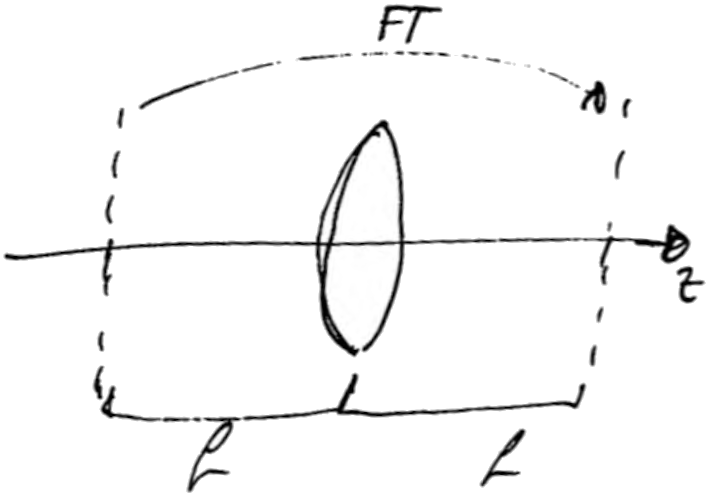
\includegraphics[width=\textwidth]{\currfiledir sketches/lens.png}
    \caption{Optical Fourier transform by a lens}
\end{marginfigure}

From geometrical optics in the paraxial approximation we know already that a lens focuses a beam  (angles $\Theta_x$, $\Theta_y$ to the optical axis) on a point 
\begin{equation}
(x,y) = (f \Theta_x, f \Theta_y)
\end{equation}
in the focal plane, where $f$ describes the focal length of the lens. A lens thus separates plane waves by their propagation direction. As in the beginning of the chapter, we can convert angles into optical frequencies and thus find that the field in the target plane $g$ is proportional the the Fourier amplitude $F$
\begin{equation}
    g(x,y) = \tilde{h} \,   F \left( \nu_x,\nu_y \right) = \tilde{h} \,  F \left( \frac{x}{\lambda d}, \frac{y}{\lambda d} \right) \quad .
\end{equation}
The remaining question is the prefactor $\tilde{h}$. If it would depend of the spatial coordinates $x$ and $y$, this would destroy the Fourier transform. To obtain $\tilde{h}$, we multiply the transfer functions of free space for the distance source plane to lens (length $d$) and lens to target plane (length $f$). And we need to multiply a transfer function for the lens, as the lens has a thickness profile $t(x,y)$ of a material with a certain index of refraction. All together one obtains\sidenote{details in \cite{SalehTeich1991}, chapter 4}
\begin{equation}
    \tilde{h}(x,y) =  \tilde{h}_0 \exp \left( 
-i \pi \frac{(x^2 - y^2)(d-f)}{\lambda^2 f}
    \right) \quad \text{with} \quad  \tilde{h}_0  = \frac{-i}{\lambda f} \, e^{ik (d+f)} \quad .
\end{equation}
This factor becomes spatially constant when the condition $d=f$ is met. A lens thus performs an optical Fourier transform between is two focal planes. In a spectrometer, the grating sits in the front focal plane of the curved mirror (acting as a lens), the detector in its back focal plane.



\section{Spatial filter}


In addition to spectrometers, the spatial filter is another important application of a lens as a Fourier transform device. We consider a so-called 4f-system, see \cite{SalehTeich1991}. All components are separated by one focal length $f$: a source plane $f$, a first lens, a filter plane $p$, a second lens and a target plane $g$. Both lenses are identical. 

\begin{marginfigure}
    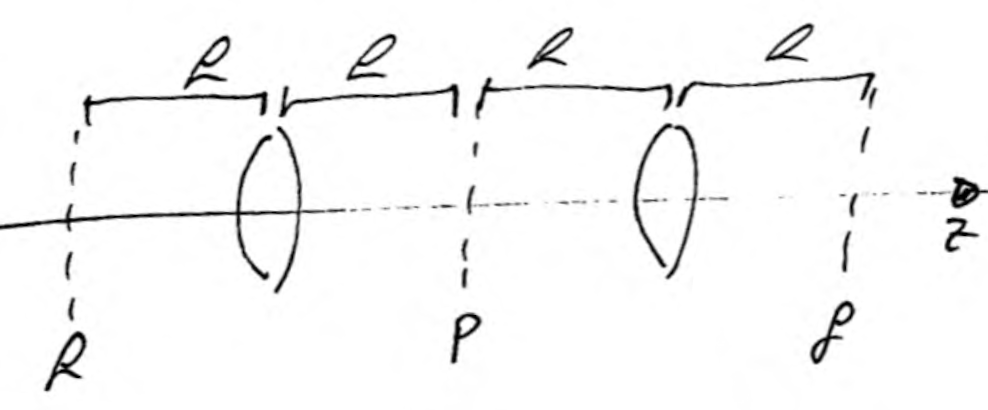
\includegraphics[width=\textwidth]{\currfiledir sketches/spatial_filter.png}
    \caption{A $4f$ system can be used as spatial filter.}
\end{marginfigure}

Let the transfer function $p$ of the filter plane be $p(x,y)=1$ for the beginning. Then the first lens Fourier transforms $f$ into $F$ in the filter plane. The filter does nothing and the second lens transforms back $F$ into $f$, so that we get in the target plane what we started with , i.e., $f=g$. Of course this make the assumption that all plane waves nicely propagate, i.e., the spatial frequencies in $f$ are small enough to cause only propagating plane waves.

The filter plane can be used to modify the Fourier components $F$. At position $x$ in the $p$ plane, only the Fourier component $\nu_x = x / (\lambda f)$ is present. We can put a mask $p(x,y)$, either just absorbing or with a complex transfer function in the filter plane. The overall transfer function of the 4f-system is then
\begin{equation}
    H(\nu_x, \nu_y) = p (\lambda f \nu_x, \lambda f \nu_y) \quad , 
\end{equation}
ignoring an overall phase factor for the propagation. 

An often used transfer function is a circular aperture. It removes all spatial frequencies above a certain threshold. In this way, one can clean up a laser beam, so that is follows the expected Gaussian profile even after transmission though many non-ideal optical elements.

The inverse filter, i.e. a opaque disc, acts as high-pass filter, increasing the edges in an optical image. A vertical slit lets only pass horizontal features in the image.



%--------------------
\printbibliography[segment=\therefsegment,heading=subbibliography]
